% !TEX root = ../report/report.tex

%%%%%%%%%%%%%%%%%%
% EE227A Project by Nathan Lam
%%%%%%%%%%%%%%%%%%


\section{Overview}

This section will review some applications using Robust PCA. Currently, most of the applications are related to computer vision. As we will show later, many images involve natural characteristic of low-rank structure, which makes Robust PCA a perfect fit to them. We will also explore some other applications that is theoretically with low-rank and sparse structure and show what we get from them. 

\section{Robust PCA Applications}

\subsection{Background modeling from surveillance video}

Video is a natural candidate for low-rank modeling, due to the correlation between frames. One of the most basic algorithmic tasks in video surveillance is to estimate a good model for the background variations in a scene. This task is complicated by the presence of foreground objects: in busy scenes, every frame may contain some anomaly. The background model needs to be flexible enough to accommodate changes in the scene, for example due to varying illumination In such situations, it is natural to model the background variations as approximately low rank. Foreground objects, such as cars or pedestrians, generally occupy only a fraction of the image pixels and hence can be treated as sparse errors.

\begin{figure}[h]
  \centering
  
\includegraphics[width=1\textwidth]{../figures/SwitchLight_original.jpg}
  \caption{Original video frames}
  \label{fig:video:original}
\end{figure}

\begin{figure}[h]
  \centering
  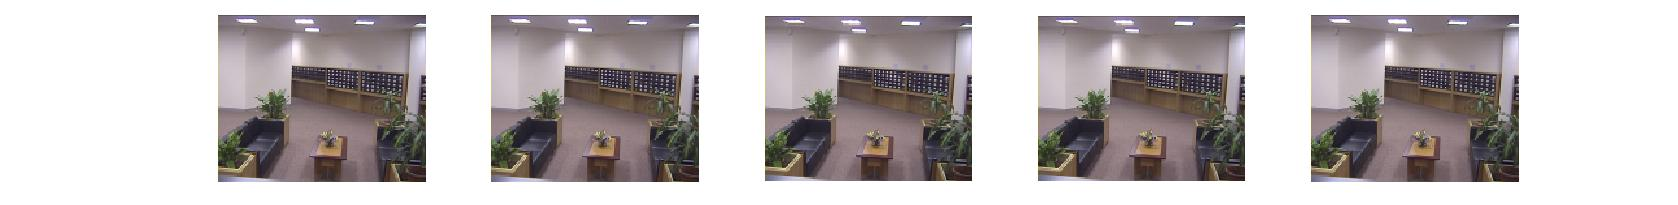
\includegraphics[width=1\textwidth]{../figures/SwitchLight_low_rank.jpg}
  \caption{Low-rank components}
  \label{fig:video:low_rank}
\end{figure}

\begin{figure}[h]
  \centering
  
\includegraphics[width=1\textwidth]{../figures/SwitchLight_sparse.jpg}
  \caption{Sparse components}
  \label{fig:video:sparse}
\end{figure}

We consider five frames from an original video, as shown in fig.~\ref{fig:video:original}, which is a scenario that  one man passes by. The resolution of each frame is $176\times144$. We first separate them into three channels (RGB). For each channel, we stack each frame as a column  of our matrix $M\in\mathbb{R}^{25344\times5}$. We decompose $M$ into low-rank components $L$ and sparse components $S$ by Robust PCA. Then we combine the three channels again to form images with low-rank component and sparse components respectively. We are using a 2GHz qual core laptop and it takes 0.92s to finish decomposition for three channels. We can find that the $L$, as shown in fig.~\ref{fig:video:low_rank}, correctly recovers the background, while $S$, as shown in fig.~\ref{fig:video:sparse}, correctly identifies the moving person.

The same setting is used into our own video that we took in UC Berkeley. The resolution in our video is $480\times640$, which is consistent with the resolution of most of the cell phone camera. Figure ~\ref{fig:video:campus:capture1} shows the result that we use 5 images which are taken every one second. It takes 15 seconds to finish. We can see that even though there are more than one person there, as long as the noise (here is the foreground) is sparse, the Robust PCA can still separate background and foreground. Since it does not consume too much time, this scenario can be considered as an application that removing wandering people when someone takes a picture.

\begin{figure}[h]
  \centering
  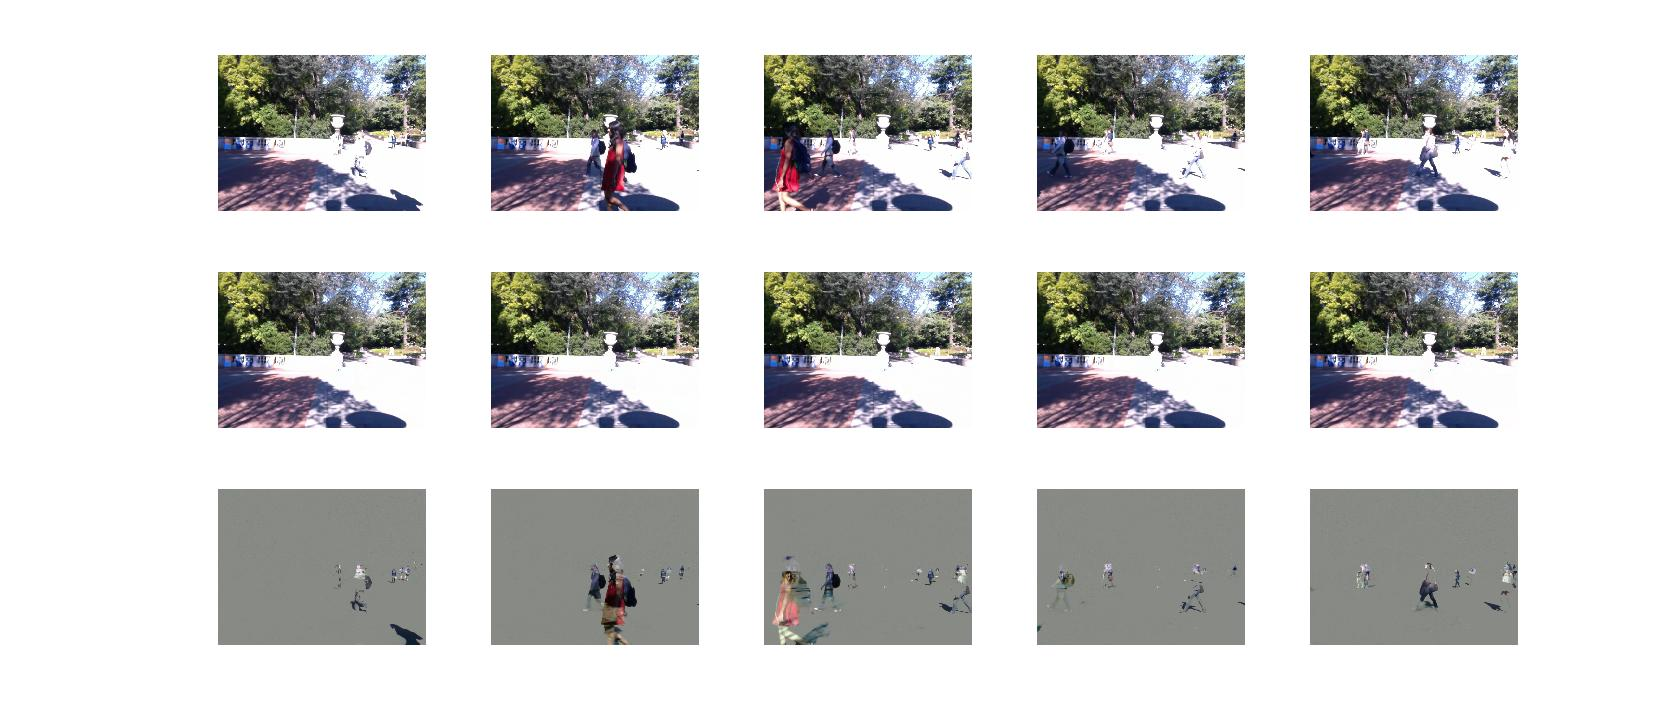
\includegraphics[width=1\textwidth]{../figures/campus_capture1.jpg}
  \caption{Perfect decomposition from campus video frames}
  \label{fig:video:campus:capture1}
\end{figure}

\begin{figure}[h]
  \centering
  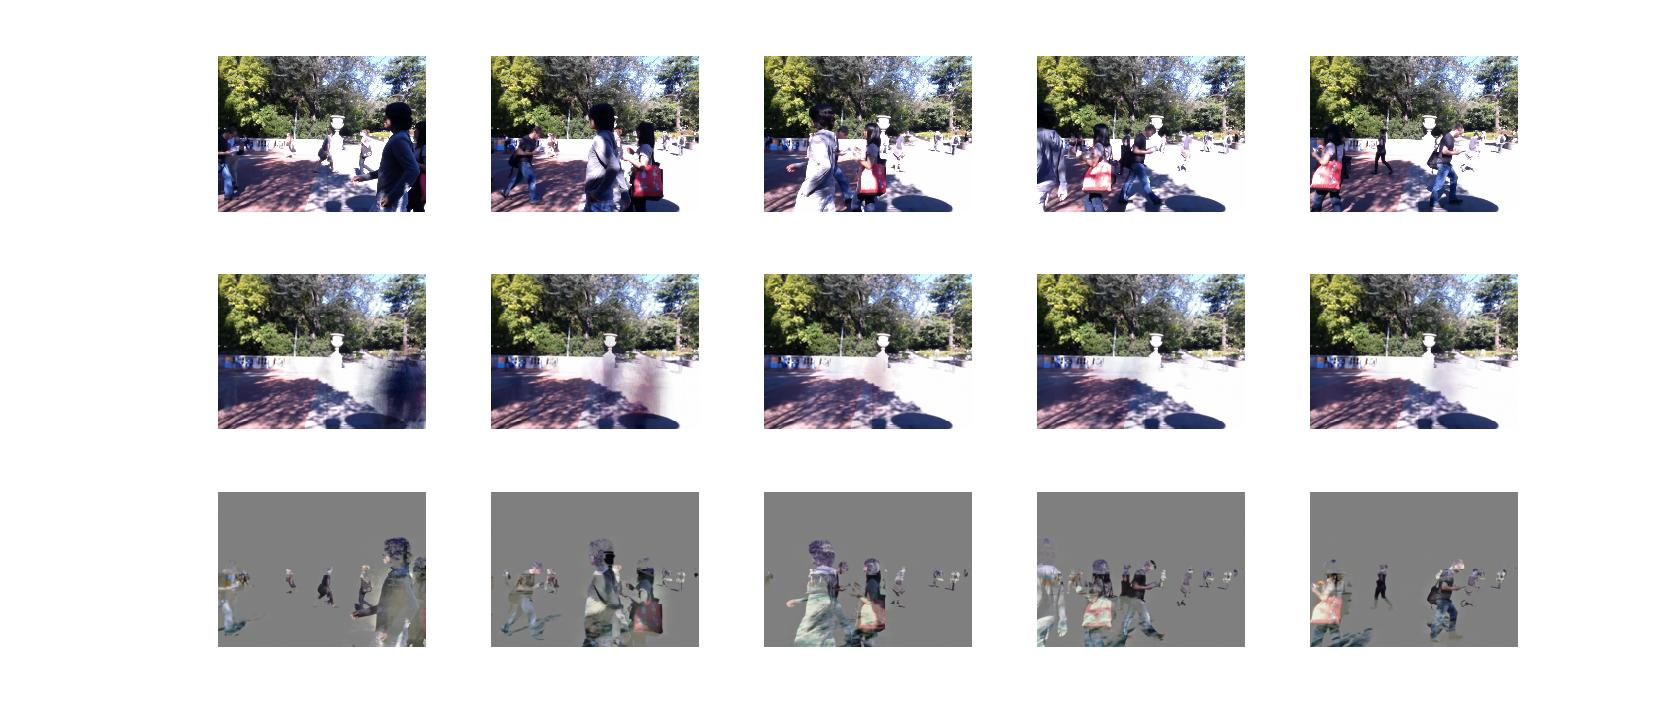
\includegraphics[width=1\textwidth]{../figures/campus_capture2.jpg}
  \caption{Imperfect decomposition from campus video frames}
  \label{fig:video:campus:capture2}
\end{figure}

Finally, we used all the frames from the 30 seconds video to run Robust PCA. We first down-sample them into $160\times214$ resolution in order to reduce the running time. We capture some frames from the resulting video. Most frames are good, but some are imperfect in terms of separating the foreground and background. We can find that in fig.~\ref{fig:video:campus:capture2}, when the foreground objects are dense, there are some "ghost" foreground people appearing in background video frames. To explain this result, we consider the following matrix:
\[
 M =
 \begin{bmatrix}
  100 & 100 & 100 & 100 & 100 \\
  100 & 100 & 100 & 100 & 100 \\
  0 & 0 & 100 & 100 & 100 \\
  100 & 100 & 100 & 100 & 100 \\
 \end{bmatrix}
\]
We can seperate $M$ into low-rank component and sparse component by Robust PCA. However, Robust PCA will favor a decomposition as:
\[
 M =
 \begin{bmatrix}
  100  & 100  & 100  & 100  & 100 \\
  100  & 100  & 100  & 100  & 100 \\
  0     &  0      & 100  & 100  & 100 \\
  100  & 100  & 100  & 100  & 100 \\
 \end{bmatrix}
 =
 \begin{bmatrix}
  100  & 100  & 100  & 100  & 100 \\
  100  & 100  & 100  & 100  & 100 \\
   34.0   & 34.0   & 36.8   & 36.8   & 36.8   \\
  100  & 100  & 100  & 100  & 100 \\
 \end{bmatrix}
 +
 \begin{bmatrix}
          0    &      0   &       0     &     0    &      0 \\
         0    &      0    &      0    &      0    &      0 \\
  -34.0  & -34.0   & 63.2   & 63.2   & 63.2 \\
         0    &      0   &       0     &     0     &     0 \\
 \end{bmatrix}
\]
such that $||L||_{*} + \lambda||S||_{1}  = 513.64$ 
rather than 
\[
 M =
 \begin{bmatrix}
  100  & 100  & 100  & 100  & 100 \\
  100  & 100  & 100  & 100  & 100 \\
  0     &  0      & 100  & 100  & 100 \\
  100  & 100  & 100  & 100  & 100 \\
 \end{bmatrix}
 =
 \begin{bmatrix}
  100  & 100  & 100  & 100  & 100 \\
  100  & 100  & 100  & 100  & 100 \\
  100  & 100  & 100  & 100  & 100 \\
  100  & 100  & 100  & 100  & 100 \\
 \end{bmatrix}
 +
 \begin{bmatrix}
          0    &      0   &       0     &     0    &      0 \\
         0    &      0    &      0    &      0    &      0 \\
  -100  & -100   & 0   & 0   & 0 \\
         0    &      0   &       0     &     0     &     0 \\
 \end{bmatrix}
\]
such that $||L||_{*} + \lambda||S||_{1}  = 536.66$ \\

From the above example, we can see that if most of the frames are corrupted in given pixels, Robust PCA hardly separates the background and foreground at those pixels perfectly. One way to solve it is to adjust the value of $\lambda$, but it is generally hard to choose a $\lambda$ that fits the entire video. Despite that, Robust PCA is still good for separating background and sparse foreground moving objects.


%%%%%%%
\subsection{Using Robust PCA in speech recognition}
Intuitively, a consistent sound would be of low-rank structure. If someone is speaking with background noise which is consistent, we would believe that we can separate a clearer speech (the sparse component) from background noise (low-rank component) via Robust PCA framework. If we get a clearer speech signal, the accuracy of speech recognition with current standard technique will increase. According to this thought, we did an experiment and try to see whether Robust PCA works in such case.

\begin{figure}[h]
  \centering
  \subfloat[clean]{\label{fig:speech:clean}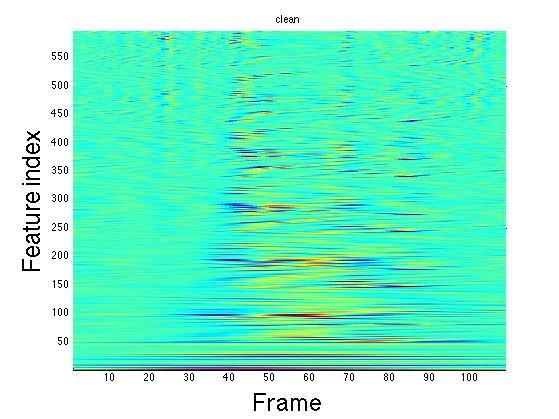
\includegraphics[width=0.5\textwidth]{../figures/speech_clean.jpg}}
  ~ %add desired spacing between images, e. g. ~, \quad, \qquad etc. (or a blank line to force the subfig onto a new line)
  \subfloat[noisy]{\label{fig:speech:noisy}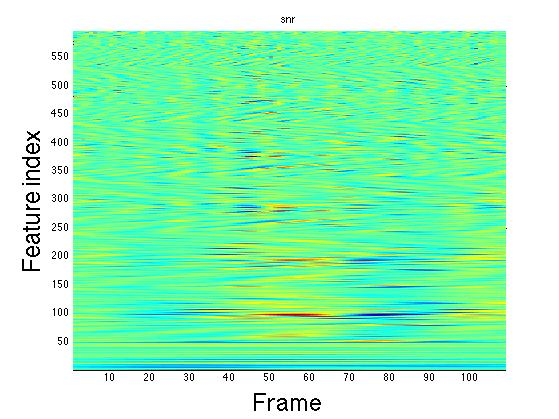
\includegraphics[width=0.5\textwidth]{../figures/speech_noisy.jpg}}
  ~ 
  \\ \subfloat[sparse]{\label{fig:speech:sparse}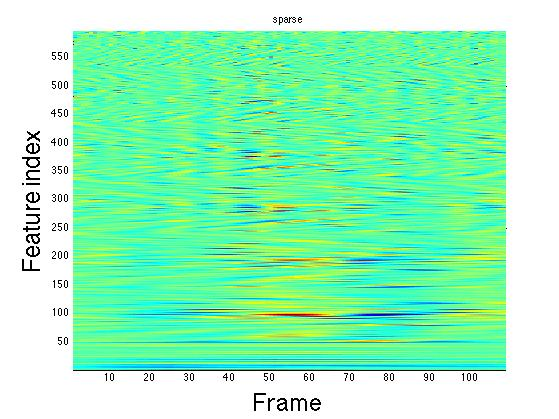
\includegraphics[width=0.5\textwidth]{../figures/speech_sparse.jpg}}
  ~
  \subfloat[low-rank]{\label{fig:speech:low_rank}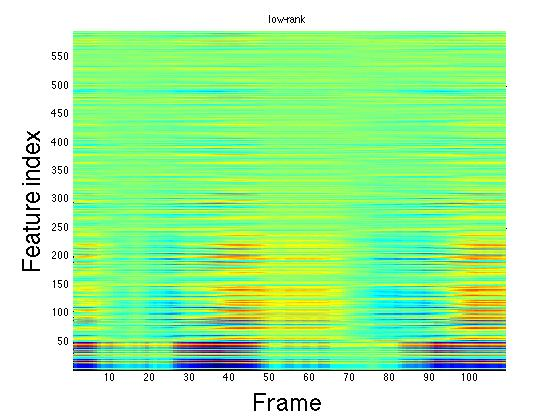
\includegraphics[width=0.5\textwidth]{../figures/speech_low_rank.jpg}}

  \caption{Speech features}
  \label{fig:speech}
\end{figure}

Figure~\ref{fig:speech:clean} shows the features of a clean speech signal, where the x-axis denotes indices of small time frames and the y-axis denote the features vectors at each frame. These features are computed by a standard method refering to \cite{}. Figure~\ref{fig:speech:noisy} shows the features domain of the same speech signal subjecting to noise with $SNR = 0$ in this case. We apply Robust PCA to decouple these features into low-rank component, as shown in fig.~\ref{fig:speech:low_rank}, and sparse component, as shown in fig.~\ref{fig:speech:sparse}. Technically, we would believe that sparse component is corresponding to our speech signal whereas low-rank component is corresponding to noise. Then we use the sparse component as new features and train a classifier via method in \cite{}. Unfortunately, comparing to the original method without  Robust PCA, we only got improvement in data set with subway noise, which we consider as the most consistent noise among the data set. In this data set, Robust PCA improve the accuracy rate with 3\% comparing to original method. For other noise, such as street noise and car noise, we both got decrease about 7\% in accuracy. One possible reason is that in the real world, most of the noise is not low-rank and they are not consistent. However, speech signal could be low-rank sometimes because there are only a limited vowels and consonants in a language, which makes Robust PCA not so suitable for de-noising.  

%%%%%%
%%%%%%
\subsection{Senators voting data analysis}
We have used Robust PCA to analyze voting data of the US senators. The data involves 100 senators voting at 542 bills around 2005 to 2008. The original data matrix is a $542\times100$ matrix with elements \{-1, 0, 1\}, representing voting for, against the bill and abstention. We first form a $100\times100$ covariant matrix and then run Robust PCA to this covariant matrix. We choose $\lambda = 1/\sqrt{10}$ as general. The rank of the low-rank component is 58 and the number of non-zero entries in sparse component is 6222. The results is shown in the following fig.~\ref{fig:vote:covariant}:


\begin{figure}[h]
  \centering
  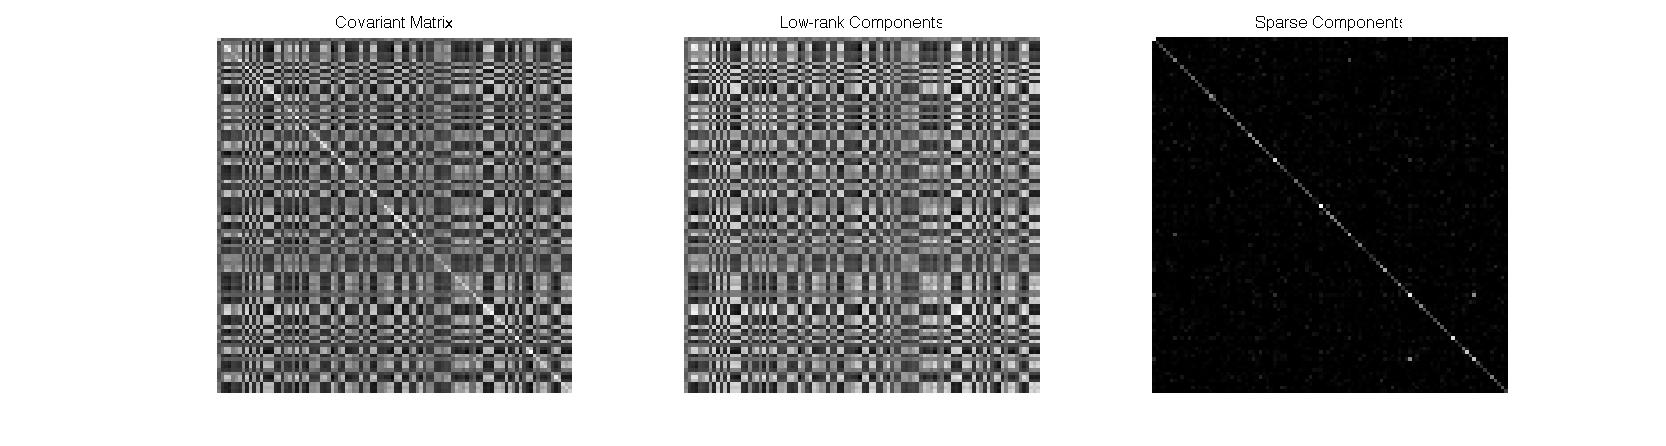
\includegraphics[width=1\textwidth]{../figures/vote_cov.jpg}
  \caption{Covariant matrix and its low-rank component and sparse component}
  \label{fig:vote:covariant}
\end{figure}

By analyzing the sparse component, we found that the sparse matrix seems to tell us some elements (i.e. senators) with strong connection. In general, the values in diagonal terms are large in sparse component because they are highly correlated. On the other hand, we could find there are some other highly correlated elements expect for the diagonal terms from the sparse matrix. We filter the value which is bigger than 0.8 in the sparse matrix expect for the diagonal terms. We found the following senators who are highly correlated in the sparse matrix: 1. (Specter, Snowe); 2. (Specter, Collins); 3. (Snowe, Collins) 4. (Jeffords, Collins) 5. (Dorgan, Conrad) 6. (Inouye, Akaka) 7. (McCain, Kyl). Interestingly, the real facts seem to match these results. First, the three Republican senators Specter, Snowe and Collins, who appear in pairs 1, 2 and 3, are always doing the same decisions, which can be shown by several reports\footnote{"The Gang of Three: Specter, Collins and Snowe" \url{http://usconservatives.about.com/b/2009/02/11/the-gang-of-three-specter-collins-and-snowe.htm}} \footnote{"NYT: Obama thanked Collins, Snowe, Specter for their �patriotism� \url{http://hotair.com/archives/2009/02/07/nyt-obama-thanked-collins-snowe-specter-for-their-patriotism/}}. Dorgan and Conrad in pair 5 are both from North Dakota. Inouye and Akaka in pair 6 are both from Hawaii. McCain and Kyl are both from Arizona. 

As shown is fig.~\ref{fig:vote:covariant:pca} and fig.~\ref{fig:vote:covariant:lr:pca}, we also compared the first two principal components in the original covariant matrix and the low-rank component. Their patterns remain similar with each other.  

\begin{figure}[h]
  \centering
  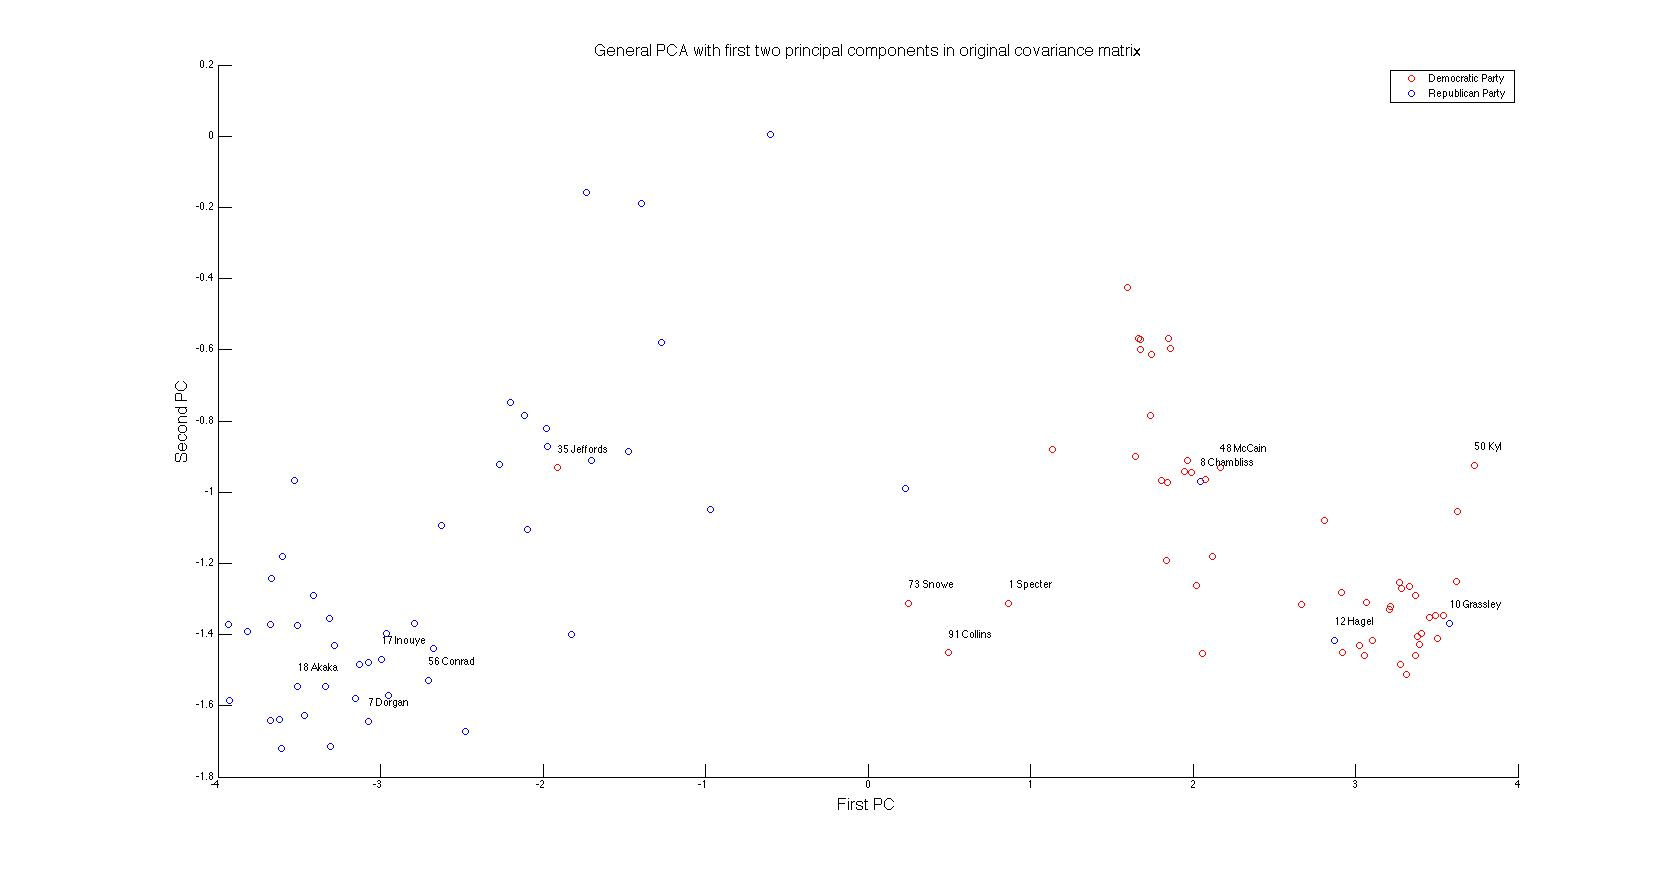
\includegraphics[width=0.85\textwidth]{../figures/vote_cov_mat_pca.jpg}
  \caption{General PCA with first two principal components in original covariant matrix}
  \label{fig:vote:covariant:pca}
\end{figure}

\begin{figure}[h]
  \centering
  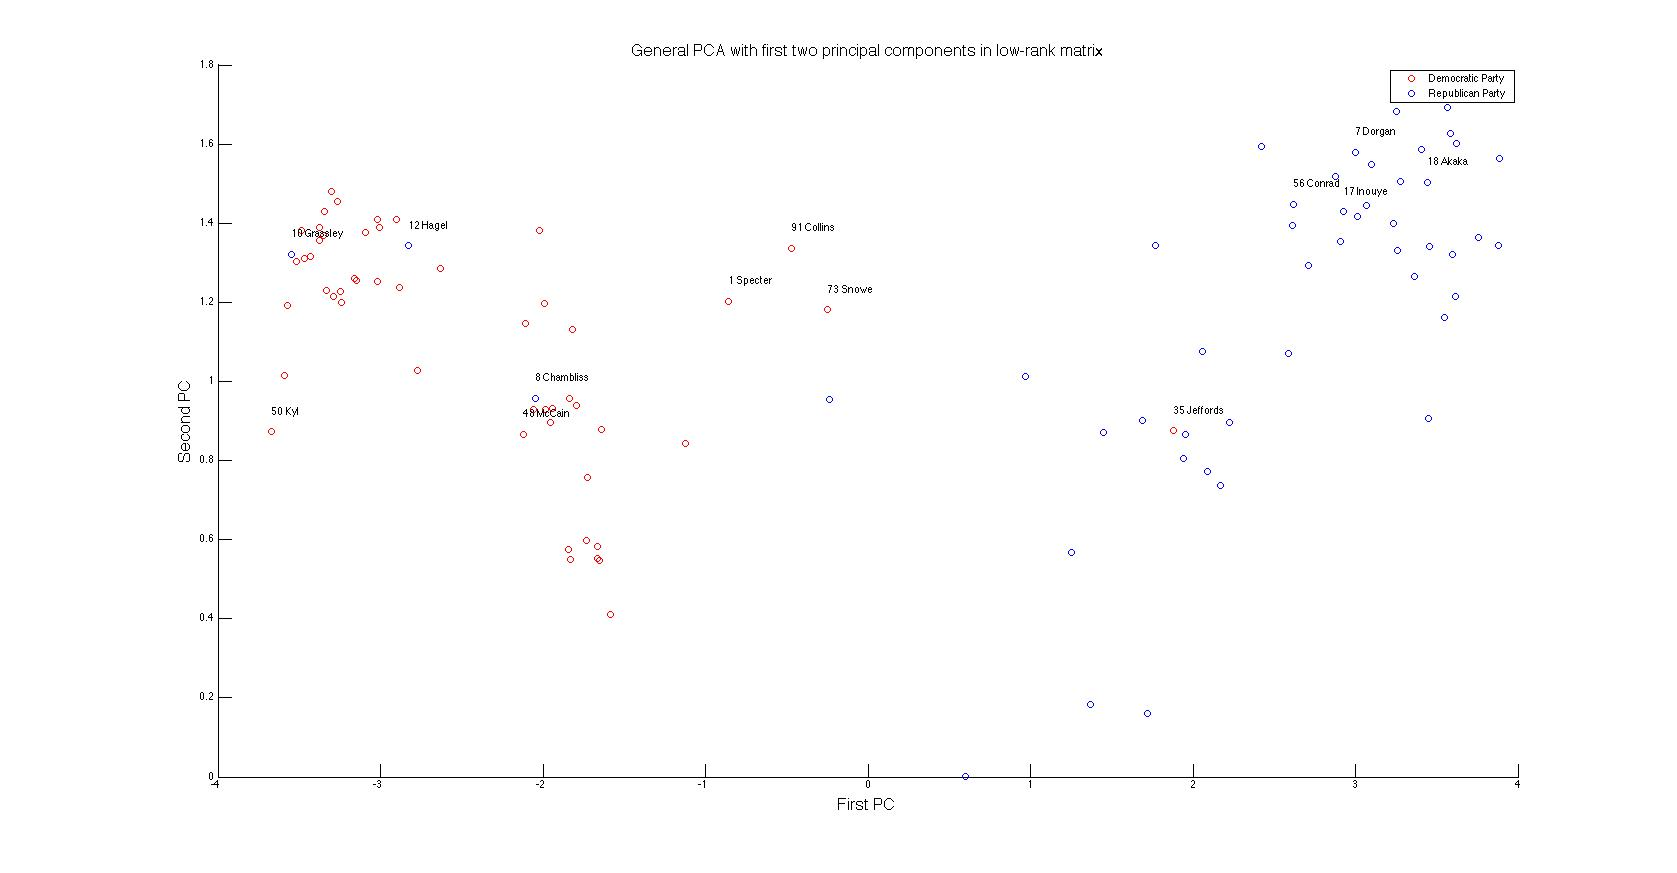
\includegraphics[width=0.85\textwidth]{../figures/vote_cov_lr_pca.jpg}
  \caption{General PCA with first two principal components in low-rank component of covariant matrix}
  \label{fig:vote:covariant:lr:pca}
\end{figure}



%%%%%
\subsection{Pre-processing of Brain-Machine Interface neural spike data}

We have used Robust PCA on some neural spike data that was collected from a monkey's brain. The Brain-Machine Interface project investigates how neural spike data can be used to interface with machines, with the ultimate goal of establishing some sort of bi-directional link (that is, to be able to control a machine through brain activity and, conversely, to ``feel'' feedback from measurements obtained by the machine). 

The particular problem we have looked at in this project was to use Robust PCA to analyze the neural spike data obtained from the motor cortex of a monkey, who was moving his arms to control a computer cursor in different directions. The assumption was that the measurements would consist of a somewhat ``low-rank'' component associated to the movement required by the particular task, and some superimposed sparse noise associated to neuron firings in the background. The data available was time-series neural spike data from a particular experiment, where the monkey had to move the cursor in 8 different directions, according to 45 degree increments. Each of the task was repeated a certain number of times. A total of 127 parallel measurement channels were available, each corresponding to a neuron (or a small number of neurons). 

As a pre-processing step, we normalized the time over the different trials for each component. The reasoning here was that the same task will correspond to the same neural firing pattern, independent of whether it was performed faster or slower\footnote{very little is known at this point about the structure of the dataset, so it was up to us to make reasonable assumptions about the data}. The next step was to group each of the trials for each of the tasks into a number of time bins, i.e. if the number of bins is~$N$ then the $i$-th bin associated to neuron~$k$ counts the number of firings of neuron~$k$ within the interval~$[(i-1)/N, i/N]$ (recall that trial time is normalized to~$1$). 

Figure~\ref{Applications:RPCAapps:BMI:raw3bins} shows the raw data after binning with 3 bins. 
%
\begin{figure}[h]
\centering
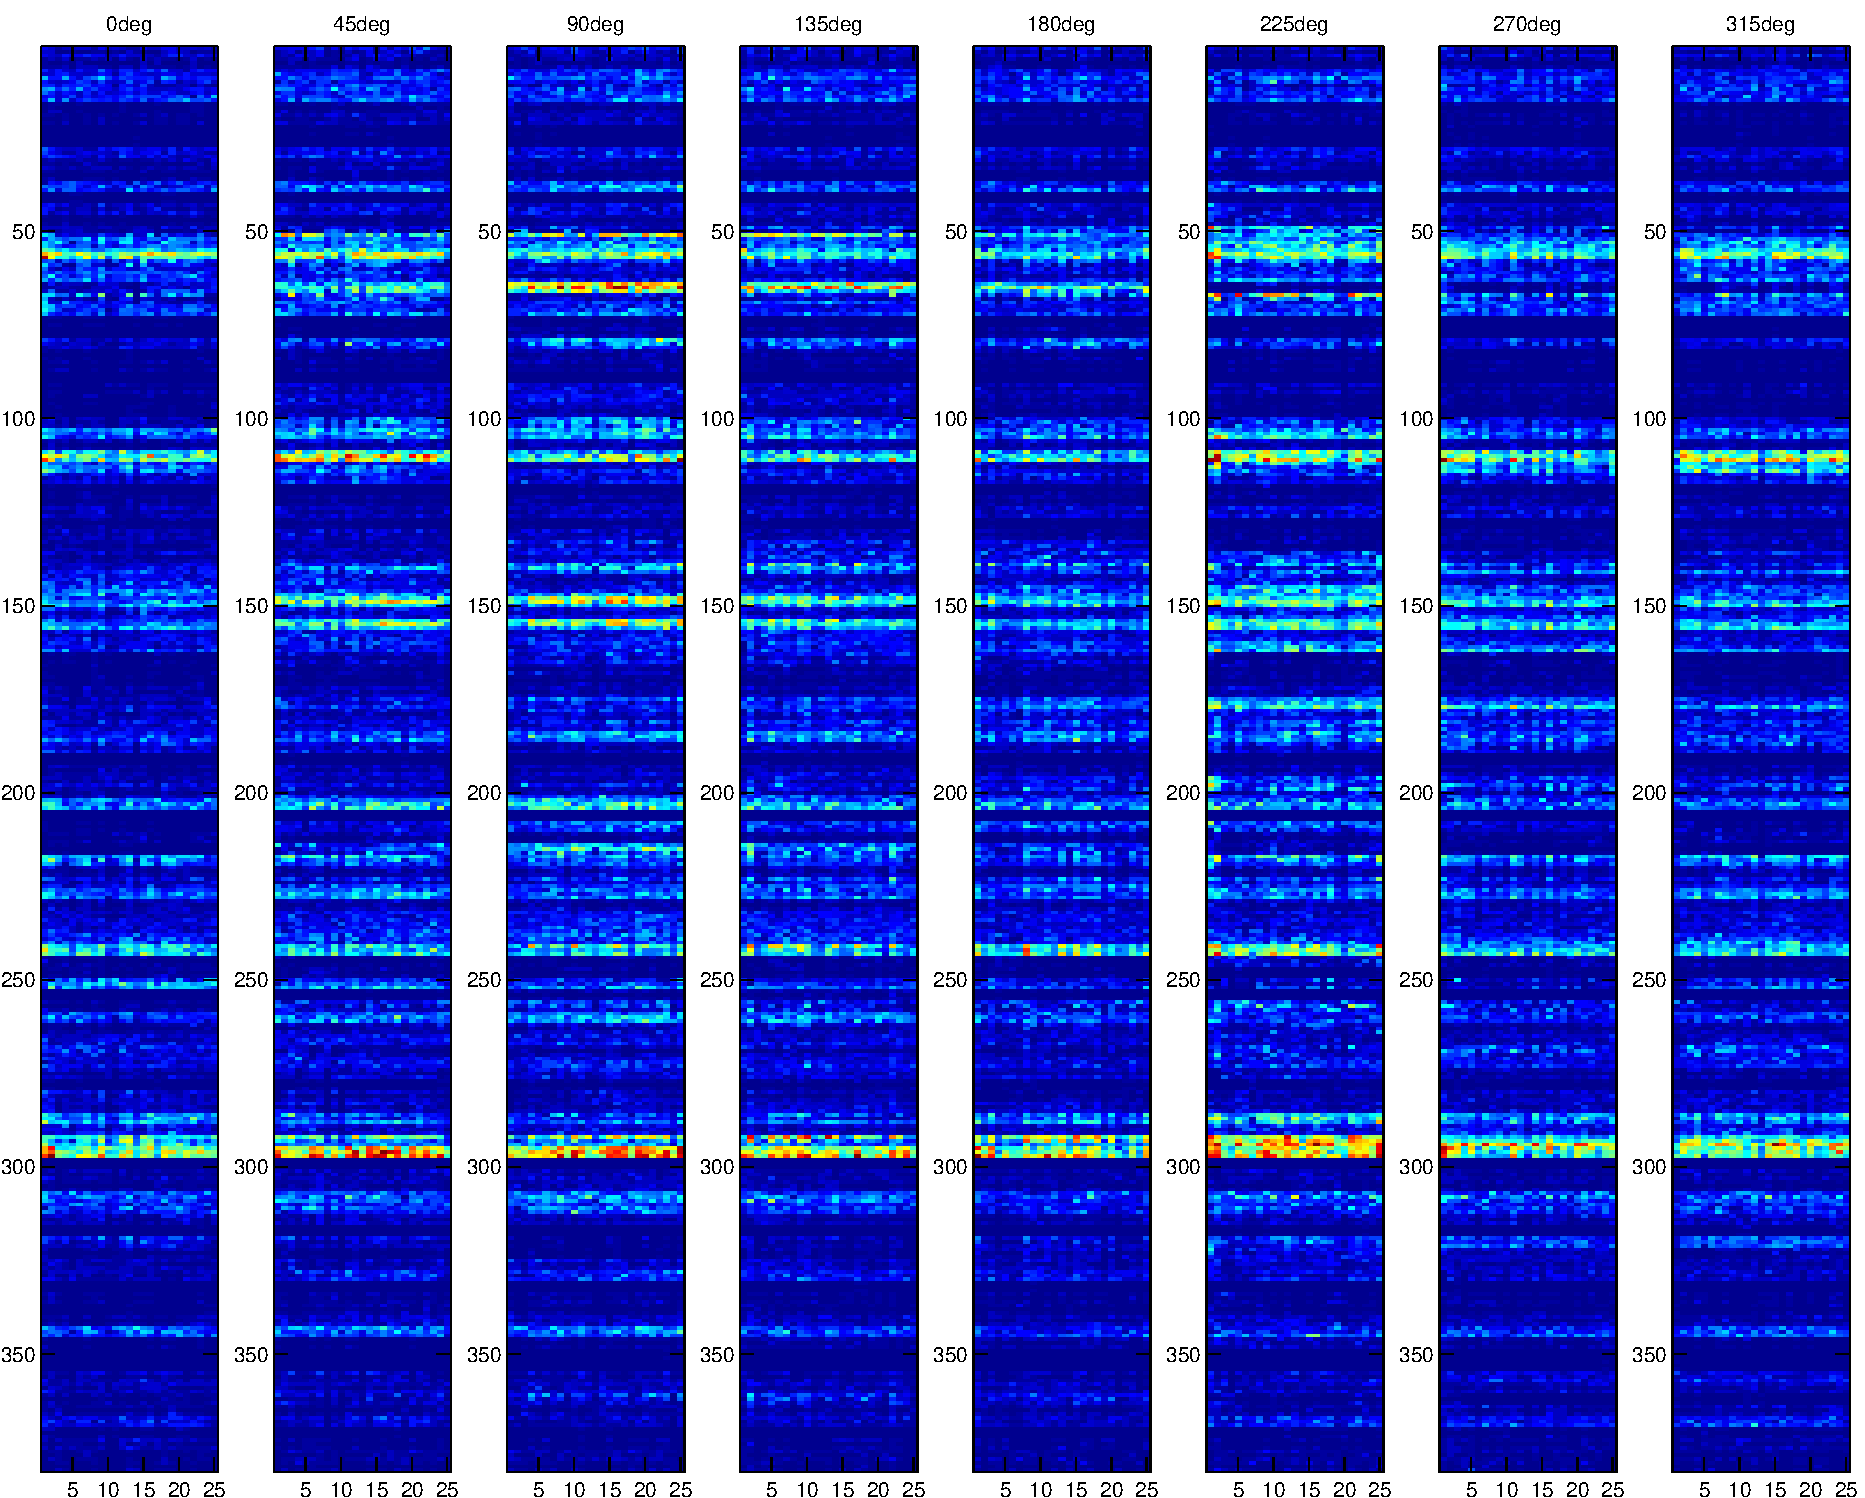
\includegraphics[width=\textwidth]{../figures/BMI_raw_3bins}
\caption{Raw (normalized and binned) neural spike data, $n_{bin}=3$}
\label{Applications:RPCAapps:BMI:raw3bins}
\end{figure}
%
here each of the 25 columns in each task represent the binned data from a single trial, where the 3 bins are stacked vertically. That is, within the large column associated to the $0\deg$ task, the first three entries of the first column correspond to the three time bins of the first neuron. The data is for 127 neurons, hence the overall matrix has $3\cdot127= 381$ rows. From the raw data in Figure~\ref{Applications:RPCAapps:BMI:raw3bins} we can already see some interesting features in the data, namely that each of the tasks seems to have its characteristic pattern. 

For each of the tasks we apply Robust PCA to the data matrix to extract low-rank and sparse components. Figure~\ref{Applications:RPCAapps:BMI:processed3bins} shows the low rank component extracted from the raw data of Figure~\ref{Applications:RPCAapps:BMI:raw3bins}. We notice that, as expected, the result is a ``filtered'' version of the raw data, in which the principal characteristics are retained while a sparse component has been removed. We think that the low-rank component in each of the tasks corresponds to the neuron firing pattern that can be directly related to the task, while the sparse component may be mis-detections, firings due to other movements, or simply sparse ``background'' firing that is always present.

%
\begin{figure}[h]
\centering
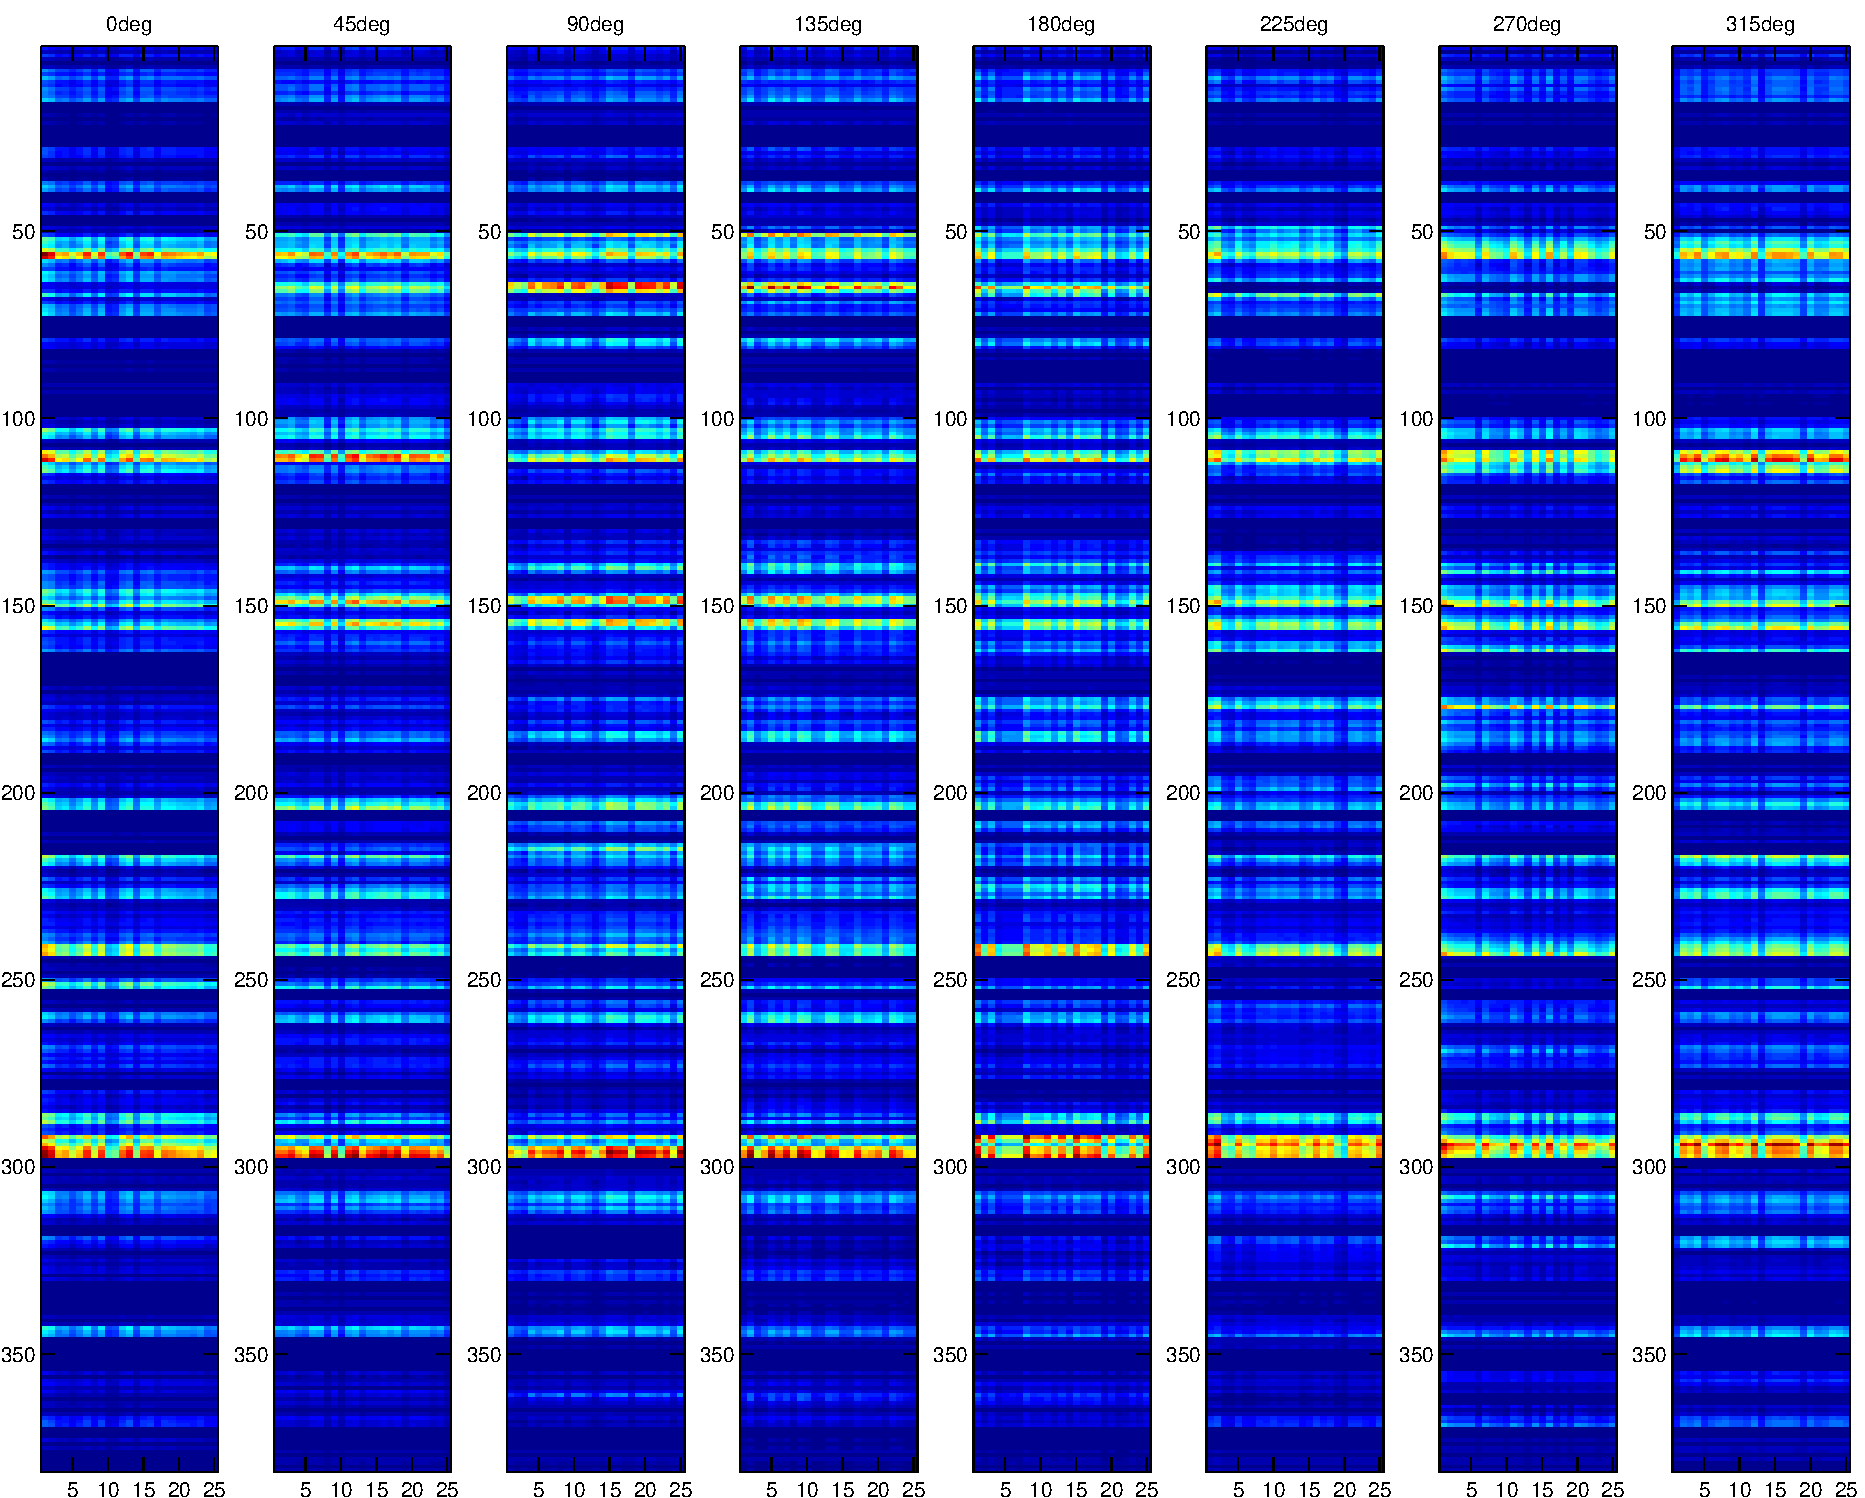
\includegraphics[width=\textwidth]{../figures/BMI_processed_3bins}
\caption{Processed neural spike data, $n_{bin}=3$}
\label{Applications:RPCAapps:BMI:processed3bins}
\end{figure}
%
For the $90\deg$ task Figure~\ref{Applications:RPCAapps:BMI:comparison90deg} shows a direct comparison of the raw data and the low-rank and sparse components obtained via Robust PCA. While for this comparably small data set the basic characteristics can be extracted visually just by looking at the matrix, this in general is not possible for high-dimensional data. One issue that we see with the available dataset is that the low rank component itself is quite sparse (since we are considering time-series data), hence some technical assumptions such as the incoherence condition will not necessarily hold. However, since not even neuroscientists have a clear understanding of what the data characteristics are and what the different patterns mean, we will not attempt to resolve this issue here. After the end of the semester we plan to learn more about the Brain-Machine interface project and, together with domain experts, to identify possible problems where Robust PCA could be used.

\begin{figure}[h]
\centering
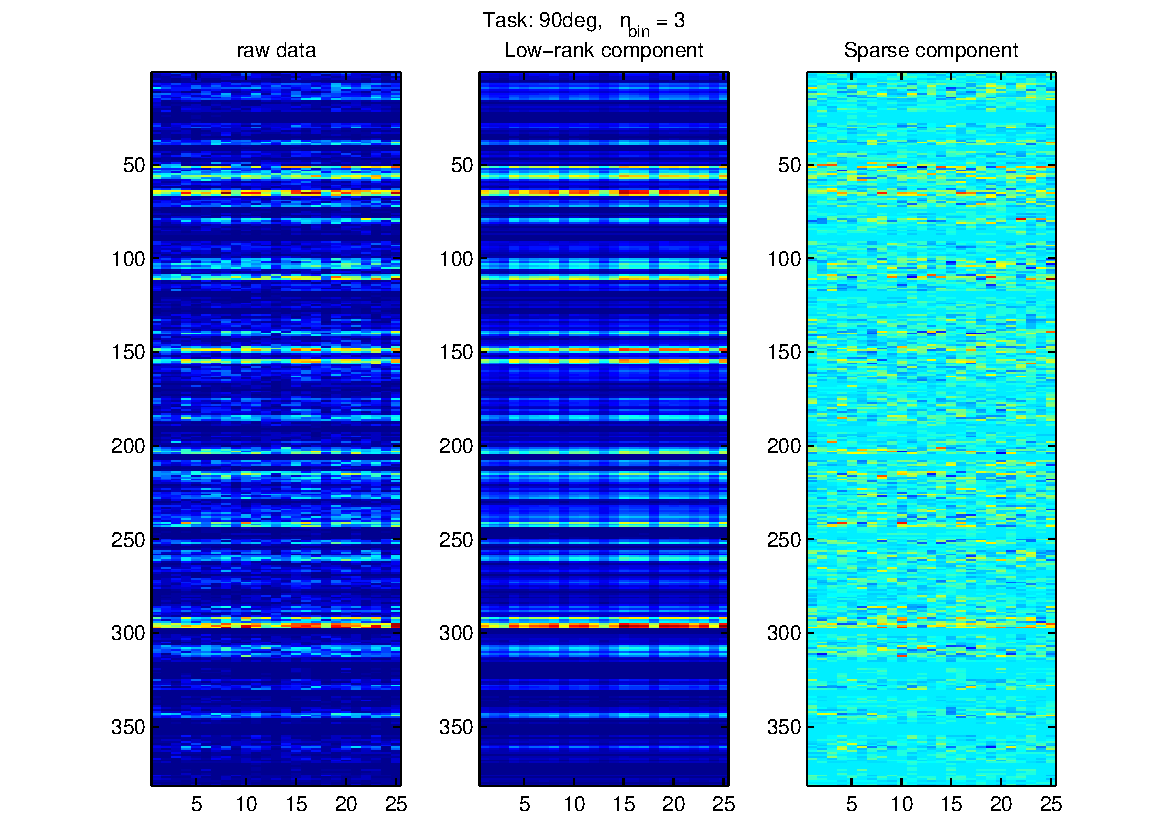
\includegraphics[width=0.95\textwidth]{../figures/BMI_comparison_90deg_3bins}
\caption{Raw data, low-rank component~$L$ and sparse component~$L$ for $90\deg$ task, $n_{bin}=3$}
\label{Applications:RPCAapps:BMI:comparison90deg}
\end{figure}

Based on the difference in neurons firing patterns between different tasks one can use machine learning techniques to predict from neural measurements which task the monkey is performing. Here Robust PCA could be used as a pre-processing step to filter out the sparse noise component. However, due to our lack of domain knowledge it is at this point unclear whether the Robust PCA framework has advantages over other and possibly simpler methods, for example a simple low-pass filters along the rows of the data matrix. Our main reason for presenting this application example here was to illustrate that Robust PCA can indeed be used as a tool to analyze interesting real data of reasonable size. 







\section{Discussion}
Robust PCA framework is a powerful tool to separate low-rank components and sparse components if we are given a combination of these two structures. However, generally most of the real world data is not directly a combination of these two structures unless the data is subjected to some kinds of transformation. One example is the data set of human faces with different expressions and illuminations. In this case, some researches have proposed some methods, RASL~\cite{Peng:2010} and TILT~\cite{Zhang:2011}, based on the original convex optimization problem in Robust PCA. They introduce transformation parameters to the original framework and by linearizing with respect to the transformation parameters, we got a new but not difficult convex problem. As long as the data is within a certain degree of transformation, the algorithms can still recover the low-rank structure and sparse structure.

We can also observe that is image data, the sparse noise is always presented as blocks. For example, the person in fig.~\ref{fig:video:sparse} appears in connected pixels, so the noise is not distributed randomly in pixels. A possible direction that can improve the separation in image data is that we can introduce a penalty term in the original optimization problem:
\begin{align}
\begin{split}
p^* = \min_{L,S} \; &||L||_{*} + \lambda \||S||_{1} + \beta\sum_{i, j\in\mathcal{N}(i)}^{} (S_{i} - S_{j})^2\\
\text{s.t.} \quad &M = L+S
\end{split}
\label{applications:discussion}
\end{align}
where $\mathcal{N}(i)$ means all the entries next to $i$ in matrix $S$. This problem is still convex so we can solve it via existing algorithm for convex optimization problems.


